\chapter{Vulnerabilità standard DDS}
\label{chvulstdndds}

In questo capitolo ci occuperemo di analizzare e comprendere 
le vulnerabilità
del middleware DDS standard OMG (Object Management Group) \cite{8469351}. 
In particolare
verrà analizzato il vettore d'attacco, il protocollo utilizzato, il bersaglio
dell'attacco e infine verrà proposta una soluzione applicabile per
mitigare i possibili attacchi. %  Nel prossimo capitolo grazie all'aiuto
% del software --inserire software-- riusciremo a capire come queste vulnerabilità
% possono essere ricreate in un ambiente simulato.
Queste falle in molti casi, possono essere sfruttate 
quando un partecipante del domain DDS è sotto il controllo di un attaccante
o quando è possibile modificare i file di configurazione delle policy QoS 
del domain.

Queste problematiche di sicurezza
riguardano la versione del DDS 1.4 con le specifiche 
dello standard OMG.

Nella Tabella~\ref{tabvulndds} viene mostrato un riassunto di tutte
le vulnerabilità presentate in questo capitolo. Come si può notare dai dati 
la soluzione più efficace per mitigare questi attacchi è utilizzare 
l'estensione DDS security che permette di crittografare le diverse
comunicazioni
scambiate tra le varie entità, rendendo più difficile per un attore 
malevolo
analizzare i contenuti dei pacchetti.






% Definizione di un colore personalizzato
\definecolor{customgray}{rgb}{0.70, 0.70, 0.70} % Grigio chiaro

% Regolazione dello spessore delle linee
\setlength{\arrayrulewidth}{1.0pt} % Spessore linee generali
% \renewcommand{\arraystretch}{1.2} % Altezza righe


\begin{table}[H]
    \centering
    \rowcolors{2}{black!5}{white}
    \resizebox{\linewidth}{!}{%
        \begin{tabular}{|c|c|c|c|c|c|}
            \hline
            \rowcolor{customgray}
            \multicolumn{1}{|>{\columncolor{customgray}}c|}{\tabularCenterstack{c}{\textbf{Tipo di}\\ \textbf{attacco}}} &
            \multicolumn{1}{>{\columncolor{customgray}}c|}{\tabularCenterstack{c}{\textbf{Vettore} \\ \textbf{attacco}}} &
            \multicolumn{1}{>{\columncolor{customgray}}c|}{\tabularCenterstack{c}{\textbf{Protoc.}/ \\ \textbf{Estens.}}} &
            \multicolumn{1}{>{\columncolor{customgray}}c|}{\tabularCenterstack{c}{\textbf{Bersaglio} \\ \textbf{nella rete}}} &
            \multicolumn{1}{>{\columncolor{customgray}}c|}{\tabularCenterstack{c}{\textbf{Software}}} &
            \multicolumn{1}{>{\columncolor{customgray}}c|}{\tabularCenterstack{c}{\textbf{Soluzione}}} \\
            \hline
            \tabularCenterstack{c}{Discovery \\ devices \cite{White2017AnII}} &
            \tabularCenterstack{c}{Verbose nature \\ of RTPS} &
            \tabularCenterstack{c}{RTPS-SDPD} &
            \tabularCenterstack{c}{Tutti i par-\\tecipanti} &
            \tabularCenterstack{c}{Sniffer \\ Python} &
            \tabularCenterstack{c}{DDS security/ \\ WireGuard} \\
            \specialrule{0.3pt}{0pt}{0pt} % Linea più spessa dopo l'intestazione
            \tabularCenterstack{c}{DDos \cite{White2017AnII}} &
            \tabularCenterstack{c}{Heartbeat \\ sequence number} &
            \tabularCenterstack{c}{RTPS} &
            \tabularCenterstack{c}{DataReader} &
            \tabularCenterstack{c}{Sniffer \\ Python} &
            \tabularCenterstack{c}{DDS security: \\ Auth Control} \\
            \specialrule{0.3pt}{0pt}{0pt} % Linea più spessa dopo l'intestazione
            \tabularCenterstack{c}{DDoS \cite{DBLP:conf/asiaccs/WangLG24}} &
            \tabularCenterstack{c}{Authentication \\ challenge} &
            \tabularCenterstack{c}{DDS security 1.1 \\ Discovery protoc.} &
            \tabularCenterstack{c}{Tutti i par-\\tecipanti} &
            \tabularCenterstack{c}{Proverif} &
            \tabularCenterstack{c}{Scadenza richieste \\ di autenticazione} \\
            \specialrule{0.3pt}{0pt}{0pt} % Linea più spessa dopo l'intestazione
            \tabularCenterstack{c}{QoS policy \cite{DBLP:conf/malware/MichaudDL18}} &
            \tabularCenterstack{c}{Policy: \\ Ownership} &
            \tabularCenterstack{c}{RTPS} &
            \tabularCenterstack{c}{DataReader} &
            \tabularCenterstack{c}{RTI \\ shapes} &
            \tabularCenterstack{c}{DDS security: \\ Access Control} \\
            \specialrule{0.3pt}{0pt}{0pt} % Linea più spessa dopo l'intestazione
            \tabularCenterstack{c}{QoS policy \cite{DBLP:conf/malware/MichaudDL18}} &
            \tabularCenterstack{c}{Policy: \\ Lifespan} &
            \tabularCenterstack{c}{RTPS} &
            \tabularCenterstack{c}{DataReader} &
            \tabularCenterstack{c}{RTI \\ shapes} &
            \tabularCenterstack{c}{Controllo per \\ Lifespan scartati} \\
            % \specialrule{0.3pt}{0pt}{0pt} % Linea più spessa dopo l'intestazione
            
            % Aggiungere altre linee

            \hline
        \end{tabular}
        }
        \caption{Riassunto delle vulnerabilità del DDS analizzate.}
        \label{tabvulndds}
    \end{table}




\section{Enumeration sniff}
% Devo spiegare il modulo discovery
Prendendo in considerazione, il protocollo RTPS,
descritto nella Sezione~\ref{Discovery module}, e il suo modulo discovery,
possiamo notare che i messaggi di default sono molto \textit{verbose}, 
scambiando le \textbf{informazioni in
chiaro} durante le comunicazioni tra i vari partecipanti \cite{White2017AnII}.
Il modulo 
discovery del protocollo RTPS a sua volta si suddivide in
altri 2 protocolli, che sono necessari per le specifiche DDS:
% (foglio 5 pag 123)
\begin{itemize}
    \item Simple Participant Discovery Protocol (SPDP).
    \item Simple Endpoint Discovery Protocol (SEDP).
\end{itemize}



\subsection{Dettagli attacco e coclusioni}
Per questo attacco ci focalizzeremo in particolare sull'SPDP che serve ad
individuare la presenza dei partecipanti al resto delle
entità nel domain. In particolar modo
il funzionamento si basa su messaggi di tipo \textit{multicast} che vengono
mandati a tutti i partecipanti attivi.
% (foglio 5 pag 125)
\cite{ddsrtps}.

L'attaccante \textit{sniffando} questi messaggi (all'interno di un domain DDS)
di tipo multicast RTPS-SPDP e
utilizzando anche un semplice script Python, potrà infatti 
vedere il loro contenuto in maniera chiara.

All'interno di un pacchetto di questo tipo possiamo trovare:
l'indirizzo IP dell'host, il prefisso GUID dell'RTPS,
la versione dell'RTPS, l'ID del venditore, i metadati 
riguardanti la sincronizzazione
ed infine il contenuto dei sottomessaggi \cite{White2017AnII}.


% \subsection{Conclusioni}
Fare una ricognizione della rete DDS senza effettuare veri e propri
attacchi di tipo attivo può essere molto utile per un attaccante che 
ha il compito di penetrare in modo attivo
una rete DDS. In molti casi tutto quello che deve fare l'attaccante
è osservare i messaggi che vengono scambiati all'interno del network.
Successivamente quando si ottengono \textbf{informazioni 
a sufficienza sarà più
facile per l'attaccante trovare altre vulnerabilità}
\cite{White2017AnII}.

Di solito questo tipo di attacco è \textbf{difficile da identificare} 
e può essere
effettuato senza lasciare tracce di nessun tipo, dato che l'attaccante non 
manda pacchetti.
Una soluzione potrebbe essere usare l'estensione DDS security o 
eseguire la connessione tra i nodi tramite un tunnel con WireGuard per crittare
le comunicazioni.



\section{Blocco DataReader tramite sequence number}

%\subsubsection{Prologo}
Il vettore di attacco si trova nel \textit{messages module} del protocollo RTPS
descritto nella Sezione~\ref{Messages module}. Questo modulo
si occupa di scambiare messaggi tra i DataReader e i DataWriter 
all'interno un domain DDS.

Per effettuare questi scambi di messaggi vengono utilizzati dei sottomessaggi,
in particolare l'HEARTBEAT e l'ACKNACK.
L'HEARTBEAT contiene al suo interno il \textit{sequence number} che tiene traccia 
del numero di aggiornamenti di un topic da parte di DataWriter, mentre
l'ACKNACK inviato da un DataReader
serve per confermare al DataWriter la ricezione di nuovi dati 
riguardo un topic.
Quando il DataReader riceve il sequence number all'interno di un HEARTBEAT
può identificare 
\textbf{se ci sono o no dei pacchetti mancanti e in caso segnalarli} al
DataWriter \cite{White2017AnII}.
Inoltre se il parametro \texttt{FINAL} è attivo in un sottomessaggio HEARTBEAT, il DataReader 
deve sempre rispondere al DataWriter con ACKNACK dopo aver ricevuto nuovi aggiornamenti.
Il DataWriter, nel frattempo, rimarrà in attesa del sottomessaggio 
ACKNACK prima di 
inviare nuovi aggiornamenti al DataReader.
Questo sistema aiuta il DataReader a rimanere sempre sincronizzato con il 
DataWriter.

I controlli del sequence number all'interno dell'HEARTBEAT 
\textbf{non sono però sufficienti} per mitigare questo attacco:
\begin{itemize}
    \item Un primo controllo viene effettuato per verificare che non ci siano 
    valori negativi;
    \item Un altro controllo serve a determinare se l'ultimo sequence number
    appena ricevuto abbia
    un valore minore rispetto a quello ricevuto in precedenza
    \cite{White2017AnII};
\end{itemize}


\subsection{Dettagli attacco e conclusioni}

Per sfruttare questa vulnerabilità l'attaccante deve utilizzare qualche 
strumento per sniffare la comunicazione tra il DataReader e il DataWriter,
intercettando così i
sottomessaggi HEARTBEAT. Dopo aver catturato un HEARTBEAT diretto verso 
un DataReader e modificato 
il suo sequence number \textbf{assegnandogli un valore molto alto}, 
l'attaccante lo rinvierà al suo destinatario originario.
Una volta ricevuto il sottomessaggio il DataReader si metterà quindi 
in attesa di un HEARTBEAT con un sequence number 
\textbf{superiore a quello appena ricevuto}. Di conseguenza il DataReader
non elaborerà più i messaggi legittimi mandati dal DataWriter,
dato che questi hanno sequence number più piccoli.
Solo un messaggio HEARTBEAT con un sequence number
maggiore a quello del DataReader farà ripristinare la sua esecuzione 
\cite{White2017AnII}.


% \subsection{Conclusioni}z
Di solito questo tipo di attacco è difficile da identificare. 
Un messaggio HEARTBEAT riguarda un solo topic, quindi il resto delle
comunicazioni che avvengono su topic differenti o anche sullo stesso topic,
ma con un DataReader diverso, non subiranno cambiamenti.
Questa falla di sicurezza può essere mitigata utilizzando l'estensione
DDS security in modo tale da crittografare i messaggi e rendere 
impossibile per l'attaccante effettuare modifiche al 
sequence number. 


\section{DDoS sfruttando estensione DDS security}
Questo vettore di attacco si trova nell'estensione del DDS chiamata
DDS security, descritto nella Sezione~\ref{DDS Security}; 
in particolare la versione utilizzata è la versione 1.1.
Il DDS security si occupa di stabilire una
connessione sicura tra i vari dispositivi della rete, impiegando 
dei plugin per effettuare: autenticazione, controllo accesso, crittografia,
login e data logging \cite{ddssecurity1.1}.

Ogni partecipante del domain DDS deve essere autenticato
dalle altre entità appartenenti allo stesso domain.
Successivamente due entità,
per iniziare una comunicazione tra di loro, devono prima
scambiarsi le chiavi private
in modo
sicuro tramite protocollo \textit{Diffie-Hellman} in modo tale da poter 
crittare i successivi
messaggi. Durante l'uso di Diffie-Hellman vengono adoperate
le \textit{challenge} (Sezione ~\ref{Processo di autenticazione}), 
che corrispondono a valori che variano nel tempo, 
inseriti durante il calcolo
della firma digitale richiesta dal protocollo. 
Queste challenge vengono utilizzate per rendere le varie sessioni 
di autenticazione uniche evitando così attacchi di tipo \textit{replay}
\cite{DBLP:conf/asiaccs/WangLG24}.

% controllare sta robbba


\subsection{Dettagli attacco e conclusioni}
L'attacco DDoS avviene durante la fase di autenticazione del
DDS security 1.1, in particolare quando un nuovo dispositivo tenta di
collegarsi alla rete e manda una richiesta di autenticazione
all'entità con cui vuole aprire una comunicazione. 
La richiesta del partecipante viene intercettata
dall'attaccante che modifica i valori della challenge crittografica 
all'interno del pacchetto. 
\textbf{Modificando ripetutamente questi valori, l'attaccante
inizia a inviare molteplici richieste crittografiche alla sua vittima.}
Il partecipante così comincerà a calcolare le firme digitali per effettuare
l'autenticazione, consumando tutte le sue risorse.
Dato che, la vittima è probabilmente un dispositivo IoT
(Internet of Things)
che non possiede di una potenza di calcolo molto elevata, si ritroverà
occupata per tutto il tempo necessario a computare diverse firme digitali
ricevute dall'attaccante, bloccando così il suo funzionamento
\cite{DBLP:conf/asiaccs/WangLG24}.


% \subsection{Conclusioni}
Questo attacco è stato scoperto con \textit{Proverif}, 
un tool che viene usato
per individuare vulnerabilità nei protocolli crittografici. 
È stato utilizzato in molti studi, ad esempio nell'analisi della 
posta elettronica certificata e nell'analisi del TLS 1.3 \cite{proverifmanual}.
% https://bblanche.gitlabpages.inria.fr/proverif/manual.pdf

Una raccomandazione per mitigare questo attacco è quello di 
cambiare delle
policy QoS impostando un tempo limite massimo per effettuare
l'autenticazione. Queste policy possono fare in modo
che i partecipanti non si trovino sopraffatti dalle 
troppe richieste di
autenticazione. Un allarme potrebbe essere utile per 
identificare possibili
tentativi DDoS di questo tipo, 
allertando così un amministratore
\cite{DBLP:conf/asiaccs/WangLG24}.






% \begin{figure}[H]
%     \centering
%     \includesvg[width=15cm,keepaspectratio]{img/Policy QoS DDS.drawio.svg}
%     \caption{Illustrazione policy QoS del DDS}\label{Mappa QoS svg}
% \end{figure}






\section{Modifica maligna OWNERSHIP\_STRENGTH}

\begin{figure}[H]
    \centering
    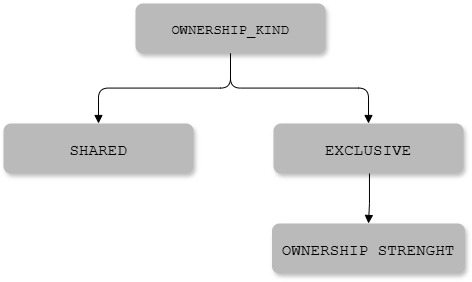
\includegraphics[width=10cm, keepaspectratio]{img/Policy QoS DDS_2.jpg}
    \caption{Illustrazione policy QoS del DDS}\label{Mappa QoS}
\end{figure}
\label{img/Policy QoS DDS_2}
% AFTER si potrebbe fare nei capitoli introduttivi una mappa che racchiuda
% i tipi di variabili che usano i QoS (int, double,.. etc) per i capitoli
% che spiegano meglio i concetti introduttivi


Questo attacco è realizzabile solo se certe policy QoS vengono
modificate durante l'esecuzione della rete, specialmente il parametro
OWNERSHIP\_KIND che gestisce \textbf{quanti DataWriter possono scrivere per un
determinato topic.} Una descrizione accurata di altre policy QoS viene 
effettuata nella Sezione~\ref{Le policy QoS nel dettaglio}.
Questo parametro può essere impostato in due modi diversi:
\begin{itemize}
    \item \textbf{SHARED:} in questo modo più DataWriter possono aggiornare le
    informazioni di un topic.
    \item \textbf{EXCLUSIVE:} solo un DataWriter può aggiornare le informazioni di un
    topic. Il DataWriter che ha il permesso di scrittura per il topic è quello
    che dispone di una OWNERSHIP\_STRENGTH con valore più alto.
\end{itemize}
% https://www.omgwiki.org/ddsf/doku.php?id=ddsf:public:guidebook:06_append:02_quality_of_service:ownership
% https://www.omgwiki.org/ddsf/doku.php?id=ddsf:public:guidebook:06_append:02_quality_of_service:ownership_strength
Nella Figura~\ref{img/Policy QoS DDS_2} viene proposto uno schema riassuntivo
delle policy QoS relative a questo attacco.
In una rete dove si adopera un OWNERSHIP\_KIND di tipo EXCLUSIVE
si consente
all'attaccante di utilizzare l'OWNERSHIP\_STRENGTH a suo favore.
Infatti è possibile far ricevere informazioni a un DataWriter
in maniera errata, dato che quest'ultimo non riceverà più dati da
una fonte affidabile 
\cite{DBLP:conf/malware/MichaudDL18}.


\subsection{Dettagli attacco e conclusioni}
L'attaccante, con un DataWriter in suo possesso all'interno di una rete DDS,
può sfruttare il fatto che il topic preso di mira può essere aggiornato
solo dal DataWriter con l'OWNERSHIP\_STRENGTH più alta.
Per effettuare questo attacco, tutto quello che serve, è 
essere a conoscenza del topic che
si vuole modificare, delle policy QoS in uso e del valore 
dell'OWNERSHIP\_STRENGTH.
L'ultimo passo è quello di \textbf{impostare la policy QoS 
nel DataWriter
dell'attaccante con una OWNERSHIP\_STRENGTH 
superiore a quella impiegata dal
DataWriter originario.}
Ora i DataReader che sono iscritti al topic bersaglio
ricevono dati dal DataWriter dell'attaccante
\cite{DBLP:conf/malware/MichaudDL18}.


% \subsection{Conclusioni}
Questa vulnerabilità è stata analizzata con l'ausilio di \textit{RTI Shapes Demo}, 
un 
software che emula una rete DDS corrispondente alle specifiche 
dello standard OMG, sviluppato da Real-Time Innovations (RTI).

L'OWNERSHIP\_KIND di tipo EXCLUSIVE è impiegata in contesti dove le
informazioni ricevute dal DataReader devono essere accurate 
dato che un singolo
DataWriter (in molti casi si tratta di un sensore) può mandare nuovi 
aggiornamenti
del topic. Se l'attaccante, dovesse riuscire a modificare i valori del 
topic, potrebbe causare molti danni,
specialmente se il DataWriter dell'attaccante riuscirà a mandare 
degli aggiornamenti
al topic senza essere scoperto
\cite{DBLP:conf/malware/MichaudDL18}.

Una soluzione utile per mitigare questo attacco potrebbe essere
l'applicazione
dell'estensione DDS security. Utilizzando i plugin relativi 
al controllo accesso,
come illustrato nella Sezione~\ref{AccessControlServicePlugin}, 
permetterà
di evitare che un attore malevolo possa modificare le policy QoS inclusa 
l'OWNERSHIP\_STRENGTH.


\section{Modifica maligna di LIFESPAN QoS}

Un'altra policy QoS che può essere usata come vettore di attacco è quella
che regola il parametro LIFESPAN. Questo parametro 
corrisponde al \textbf{tempo limite massimo 
di validità per la
lettura di pacchetti} da parte di un DataReader. Per determinare se un pacchetto
di un topic è scaduto viene utilizzato il \textit{timestamp} di creazione
aggiungendo il valore del LIFESPAN impostato; se questo risultato chiamato 
\textit{expiration time} risulterà
superiore all'orario durante la ricezione del DataReader, allora il pacchetto
ricevuto sarà ancora valido. 
Per funzionare, gli orologi interni del DataWriter e del DataReader
devono essere sincronizzati tra di loro.

Un'altra policy da considerare riguarda l'affidabilità (RELIABILITY),
che può essere impostata in due
modi, dei dati riguardanti un topic :
\begin{itemize}
    \item RELIABLE: questa impostazione costringe il DataReader a farsi
    ritrasmettere dal DataWriter i pacchetti mancanti o ricevuti in maniera errata.
    In questo modo le informazioni del DataReader saranno sempre corrette anche
    se non sempre aggiornate in tempo reale.
    \item BEST-EFFORT: l'impostazione predefinita non consente il recupero
    dei pacchetti mancanti o corrotti
    del DataReader, quindi, quest'ultimo potrebbe anche perdere dei pacchetti 
    che gli sono stati inviati \cite{dds1.4}.
\end{itemize}
% https://www.omgwiki.org/ddsf/doku.php?id=ddsf:public:guidebook:06_append:02_quality_of_service:reliability
Se il LIFESPAN dei pacchetti, contenenti i dati del topic,
viene impostato con valori molto piccoli, si verificheranno problemi di comunicazione
tra DataWriter e DataReader, dato che non sarà possibile effettuare la lettura di 
certi pacchetti inviati. Impostando il valore RELIABLE tra le policy QoS con
RELIABILITY sarà possibile mitigare 
solo parzialmente questa vulnerabilità
\cite{DBLP:conf/malware/MichaudDL18}.

% https://www.omgwiki.org/ddsf/doku.php?id=ddsf:public:guidebook:06_append:02_quality_of_service:lifespan


\subsection{Dettagli attacco e conclusioni}
Avendo sotto controllo i parametri LIFESPAN e RELIABLE, l'attaccante modificherà le
policy dei DataWriter in modo tale da \textbf{avere il valore LIFESPAN molto piccolo.} 
Così
facendo, i pacchetti spediti dal publisher 
arriveranno già scaduti al DataReader,
rendendoli inutilizzabili. In certi casi il pacchetto che deve essere inviato
viene distrutto dallo stesso DataWriter 
all'interno della sua coda prima dell'invio. 
Questa falla di sicrezza è stato verificata configurando il valore di
LIFESPAN < 80ms dove si è visto che nessun pacchetto raggiunge il DataReader.
Se si aumenta il valore tra gli 80ms e i 100ms già si 
può notare che dei pacchetti
vengono letti con successo dal DataReader, mentre altri vengono eliminati prima
della lettura. Infine impostando un valore LIFESPAN >= 120ms si può notare che
la comunicazione tra publisher e subscriber avverrà senza nessun problema.

Un dettaglio da aggiungere è che se si imposta la policy
dell'affidabilità (RELIABILITY) con la flag RELIABLE, i millisecondi necessari
del LIFESPAN per compromettere le comunicazioni tra DataReader e DataWriter
devono essere \textit{moltiplicati per un fattore di 0.01}. Quindi, ad esempio se si
ottiene un completo annullamento delle comunicazioni con un LIFESPAN < 80ms
utilizzando la RELIABILITY di tipo BEST-EFFORT, per ottenere lo stesso
risultato con RELIABILITY di tipo RELIABLE dobbiamo impostare un
LIFESPAN < 0.8ms
\cite{DBLP:conf/malware/MichaudDL18}.

% \subsection{Conclusioni}
Anche questo test è stato dimostrato con RTI Shapes Demo che 
implementa una
soluzione DDS di RTI corrispondente alle specifiche dello standard OMG.
Inizialmente molte reti DDS hanno impostato la RELIABILITY
di tipo BEST-EFFORT che è l'impostazione predefinita,
in modo tale da rendere possibili comunicazioni di tipo real-time.
Quindi nella maggior parte
dei casi l'attore malevolo 
non si deve preoccupare di modificare questo parametro.

Una possibile soluzione consiste nell'implementare qualche tipo di controllo
in modo tale da avvertire un operatore umano se molti pacchetti vengono
scartati perché arrivati con un LIFESPAN scaduto. Questo controllo potrebbe
essere anche utile, nel caso in cui il DataWriter e il DataReader si trovassero
distanti fisicamente tra di loro, per verificare la qualità del collegamento
\cite{DBLP:conf/malware/MichaudDL18}.


